\documentclass[10pt]{article}
\usepackage{fontspec}
\setmainfont{Times New Roman}
\newfontfamily{\headingfont}{Times New Roman}
\usepackage[utf8]{inputenc}
\usepackage{xcolor}
\usepackage{authblk}
\usepackage{graphicx}
\usepackage[a4paper, total={6in, 8in}]{geometry}
\usepackage{float}
\usepackage{natbib}
%\usepackage[T1]{fontenc}
\usepackage{nomencl}
\usepackage{titlesec}

\titleformat{\section}
  {\normalfont\fontsize{10}{10}\sffamily\bfseries}
  {\thesection}
  {1em}
  {}
\titleformat{\subsection}
  {\normalfont\fontsize{10}{10}\sffamily\bfseries}
  {\thesubsection}
  {1em}
  {}


\makenomenclature
\usepackage[style=authoryear-ibid,backend=biber]{biblatex}
\addbibresource{references.bib}% Syntax for version >= 1.2

\title{ A semi-empirical method for predicting roll damping based on machine learning }
\renewcommand\Authfont{\small}
\renewcommand\Affilfont{\small}
\author[1,2]{Martin Alexandersson}
\author[1]{Wengang Mao}
\author[1]{Jonas W Ringsberg}
\affil[1]{Dept. of Mechanics and Maritime Sciences, Chalmers University of Technology, 41296 Gothenburg, Sweden}
\affil[2]{SSPA Sweden AB, 41296 Gothenburg, Sweden}
\affil[ ]{\textit {maralex@chalmers.se}}
\date{}

\begin{document}
\begin{figure}
    \centering
    \includegraphics[width=\columnwidth]{figures/ICSOS_logo.png}
\end{figure}

\maketitle
\thispagestyle{empty}

\vspace*{-0.5in}
{\footnotesize
\noindent\rule{\columnwidth}{0.4pt}
\section*{Abstract}\label{se:abstract}

Semi-empirical methods such as the Ikeda’s method is widely used to predict roll damping for practical purposes. Recent work has shown that the applicability and accuracy of Ikeda’s method for modern hull forms are somewhat uncertain which is very unfortunate, especially for analysis of parametric roll. 
%A small error in the roll damping prediction can make the difference between having no parametric roll and disaster.
This paper presents a new semi-empirical method as a complement to the simplified Ikeda's method. The new method has been developed using a regression based approach on a roll damping database built by performing parameter identification of roll decay model tests. 
The new method is estimated to have higher accuracy than the simplified Ikeda's method which has been investigated using cross validation on the roll damping database. The paper also suggests a lower limit for the ship draughts where the simplified Ikeda's method can be used.


\noindent {\scriptsize \emph{Keywords}: Roll damping; Roll decay; Ikeda’s method; Simplified Ikeda’s method; Ship motions; Parameter identification technique.}
}
\newline
\noindent\rule{\columnwidth}{0.4pt}
%\newpage
%\tableofcontents
%\newpage

\section{Introduction}
\label{se:introduction}

In the second generation of intact stability criteria, the IMO has addressed the importance of ships having sufficient roll damping to avoid parametric roll and large roll motions in dead ship condition as well as excessive acceleration \parencite{imo_finalization_2016}. 
Since the scale effect of the damping is mainly associated with the skin friction on ship hulls and the friction only contributes very little to a full scale ship's total roll damping, experimental tests is a widely accepted method to estimate a ship's roll damping \parencite{imo_1200_2006}. A lot of research activities have been put on methods to estimate roll damping from experimental tests. For example, \parencite[]{hua_approximation_2011} investigated a second order oscillator model to approximate the a ship's roll damping based on both experiments at different scales and numerical calculations. \parencite{soder_ikeda_2019} presented unique experimental set-ups in model scale and full-scale to evaluate roll damping properties from the test results. 
As the rapid increase of computation capability, the CFD methods have also been used to calculate the roll damping as in \parencite{kristiansen_experimental_2014} and \parencite{henry_peter_piehl_ship_2016}.  

However, in the early stage of ship design, when only limited information is available, such as the ship's principal dimensions and the basic hull geometry, computational fluid dynamics or experimental model tests are not feasible options.
Therefore, simpler methods are widely used. Simpler strip theory methods can give quite accurate prediction of a ship's pitch, heave, sway and yaw motions, but often overestimates the roll motions because of significant viscous effects on the roll damping \parencite{kawahara_simple_2011}. Therefore other methods are used to obtain the roll damping at early design stage. Several semi-empirical methods were proposed in the late 70th as described by  \parencite{himeno_prediction_1981}. The most recognize method was developed in a series of research articles \parencite{ikeda_roll_1978,ikeda_eddy_1978,ikeda_roll_1979,ikeda_components_1978,ikeda_velocity_1979}, often referred to as the Ikeda's method. This method divides the roll damping into five damping components, i.e., the friction component, the eddy component, the lift component, the wave component and the bilge keel component. This semi-empirical method is also recommended by \parencite{ittc_ittc_2011}. As reported by  \parencite{kawahara_simple_2011} and \parencite{soder_ikeda_2019}, Ikeda's method may not work well for unconventional ships, such as container ship and PCTC with pronounced flare bow and stern structures. In addition, the rather widely used simplified Ikeda's method \parencite{kawahara_simple_2011} (SI-method) was constructed by a series of old ship hulls, while it might not give a fare estimation of roll damping of today's much optimized ship hull forms.
Concerning that the SI-method method may considerably underestimate the eddy making component of damping of full hull forms, \parencite{rudakovic_application_2017} adjusted the simplified Ikeda’s method and  extended its application to stability analysis of inland ships.

The main objective of this paper is to investigate the accuracy of the SI-method for modern ships using more than 250 roll decay tests conducted at SSPA during the past 15 years. The second objective is to investigate if the accuracy of the SI-method can be improved for modern ships or if a complete new method is needed. 

To make the completeness of the paper section \ref{se:methods_for_prediction_and_analysis} presents the basic governing equations of roll motions and how roll damping can be obtained from roll decay tests and the SI-method. 
The roll decay test database is presented in section \ref{se:accuracy_SI_method}, as well as the roll damping estimated by the system identification techniques as damping references, which are compared with the SI-method to identify weaknesses and strengths of this method. Section \ref{se:correction_SI_method} proposes a new regression-based method to improve the accuracy of roll damping in comparison with the SI-method. Conclusions are given in section \ref{se:conclusions}.  

\mbox{}
\nomenclature{$\displaystyle T$}{Mean draught\nomunit{$m$}}
\nomenclature{$\displaystyle C_{5A}$}{\nomunit{$$}}
\nomenclature{$\displaystyle \rho$}{water density\nomunit{$kg/m3$}}
\nomenclature{$\displaystyle B_{e}$}{Equivalen linearized damping\nomunit{$Nm/(rad/s)$}}
\nomenclature{$\displaystyle B_{L}$}{Hull lift roll damping\nomunit{$Nm/(rad/s)$}}
\nomenclature{$\displaystyle L_{pp}$}{ship perpendicular length\nomunit{$m$}}
\nomenclature{$\displaystyle Disp$}{displacement\nomunit{$m**3$}}
\nomenclature{$\displaystyle B_{1 hat}$}{Nondimensional damping\nomunit{$-$}}
\nomenclature{$\displaystyle \omega_{0}$}{\nomunit{$$}}
\nomenclature{$\displaystyle C_{1A}$}{\nomunit{$$}}
\nomenclature{$\displaystyle B_{F}$}{Friction roll damping\nomunit{$Nm/(rad/s)$}}
\nomenclature{$\displaystyle B_{2 hat}$}{Nondimensional damping\nomunit{$-$}}
\nomenclature{$\displaystyle \delta$}{\nomunit{$$}}
\nomenclature{$\displaystyle B_{BK}$}{Bilge keel roll damping\nomunit{$Nm/(rad/s)$}}
\nomenclature{$\displaystyle B_{3A}$}{\nomunit{$$}}
\nomenclature{$\displaystyle B_{e hat 0}$}{Nondimensional damping\nomunit{$-$}}
\nomenclature{$\displaystyle A_{44}$}{General roll inertia\nomunit{$kg*m**2$}}
\nomenclature{$\displaystyle \omega$}{Frequency of external moment\nomunit{$rad$}}
\nomenclature{$\displaystyle \zeta$}{\nomunit{$$}}
\nomenclature{$\displaystyle B_{1A}$}{\nomunit{$$}}
\nomenclature{$\displaystyle BK_{L}$}{Bilge keel length\nomunit{$m$}}
\nomenclature{$\displaystyle OG$}{Distance from roll axis to still water level\nomunit{$m$}}
\nomenclature{$\displaystyle B_{1}$}{\nomunit{$$}}
\nomenclature{$\displaystyle D$}{\nomunit{$$}}
\nomenclature{$\displaystyle B_{44}$}{Total roll damping\nomunit{$Nm/(rad/s)$}}
\nomenclature{$\displaystyle B_{3}$}{\nomunit{$$}}
\nomenclature{$\displaystyle C_{b}$}{Block coefficient\nomunit{$-$}}
\nomenclature{$\displaystyle BK_{B}$}{Bilge keel height\nomunit{$m$}}
\nomenclature{$\displaystyle C_{1}$}{\nomunit{$$}}
\nomenclature{$\displaystyle d$}{\nomunit{$$}}
\nomenclature{$\displaystyle C_{5}$}{\nomunit{$$}}
\nomenclature{$\displaystyle C_{3}$}{\nomunit{$$}}
\nomenclature{$\displaystyle B_{E}$}{Eddy roll damping\nomunit{$Nm/(rad/s)$}}
\nomenclature{$\displaystyle \phi_{a}$}{Initial roll amplitude\nomunit{$rad$}}
\nomenclature{$\displaystyle B_{44 hat}$}{Nondimensional damping\nomunit{$-$}}
\nomenclature{$\displaystyle C_{3A}$}{\nomunit{$$}}
\nomenclature{$\displaystyle g$}{acceleration of gravity\nomunit{$m/s**2$}}
\nomenclature{$\displaystyle t$}{\nomunit{$$}}
\nomenclature{$\displaystyle V$}{Ship speed\nomunit{$m/s$}}
\nomenclature{$\displaystyle B_{2A}$}{\nomunit{$$}}
\nomenclature{$\displaystyle B_{e hat}$}{Nondimensional damping\nomunit{$-$}}
\nomenclature{$\displaystyle B_{W}$}{Wave roll damping\nomunit{$Nm/(rad/s)$}}
\nomenclature{$\displaystyle A_{0}$}{Mid ship area coefficient\nomunit{$-$}}
\nomenclature{$\displaystyle C$}{\nomunit{$$}}
\nomenclature{$\displaystyle m$}{mass of ship\nomunit{$kg$}}
\nomenclature{$\displaystyle B_{2}$}{\nomunit{$$}}
\nomenclature{$\displaystyle GM$}{metacentric height\nomunit{$m$}}
\nomenclature{$\displaystyle \omega_{hat}$}{Nondimensional roll frequency\nomunit{$-$}}
\nomenclature{$\displaystyle beam$}{ship beam\nomunit{$m$}}
\nomenclature{$\displaystyle B_{e factor}$}{Nondimensional damping\nomunit{$-$}}

\printnomenclature

\section{Methods for prediction and analysis of roll damping}
\label{se:methods_for_prediction_and_analysis}

\section{Accuracy of current methods for predicting roll damping}
\label{se:accuracy_SI_method}
Some studies for instance \parencite{soder_assessment_2019} show that the Ikeda's method is not capable to accurately predict the roll damping for some modern ship cases. The SI-method being the simplified version of Ikeda's method most likely inherits its problems but also introduces some extrapolation errors as reported by \parencite{rudakovic_application_2017}. In the following, 227 existing roll decay model tests conducted at SSPA Maritime Dynamics Laboratory are used to validate the SI-method. The comparison will help to identify the drawbacks and improvement potentials of the SI-method. It aims at further developing this method to increase its accuracy based on the large test database through some statistical regression analysis.

Prior to the validation the behaviour of the SI-method was studied by varying the input parameters between minimum and maximum values in database around a point "reference ship" with values in the middle of the input boundaries (Eq. \ref{eq:SI_limits}) (see figure \ref{fig:SI_sensitivity}). It can be seen that the wave damping $B_W$ increases a lot with the absolute value of $OG/T$. It can also be seen the the wave damping has an enormous increase when the beam to draught ratio exceeds the input boundary, which seems to be the case for at least one third of the roll decay tests. It can also be noted that most of the ships in the database have midsection coefficients $A_0$ and bilge keel heights that exceed the limit. 

\begin{figure}[H]
    \centering
    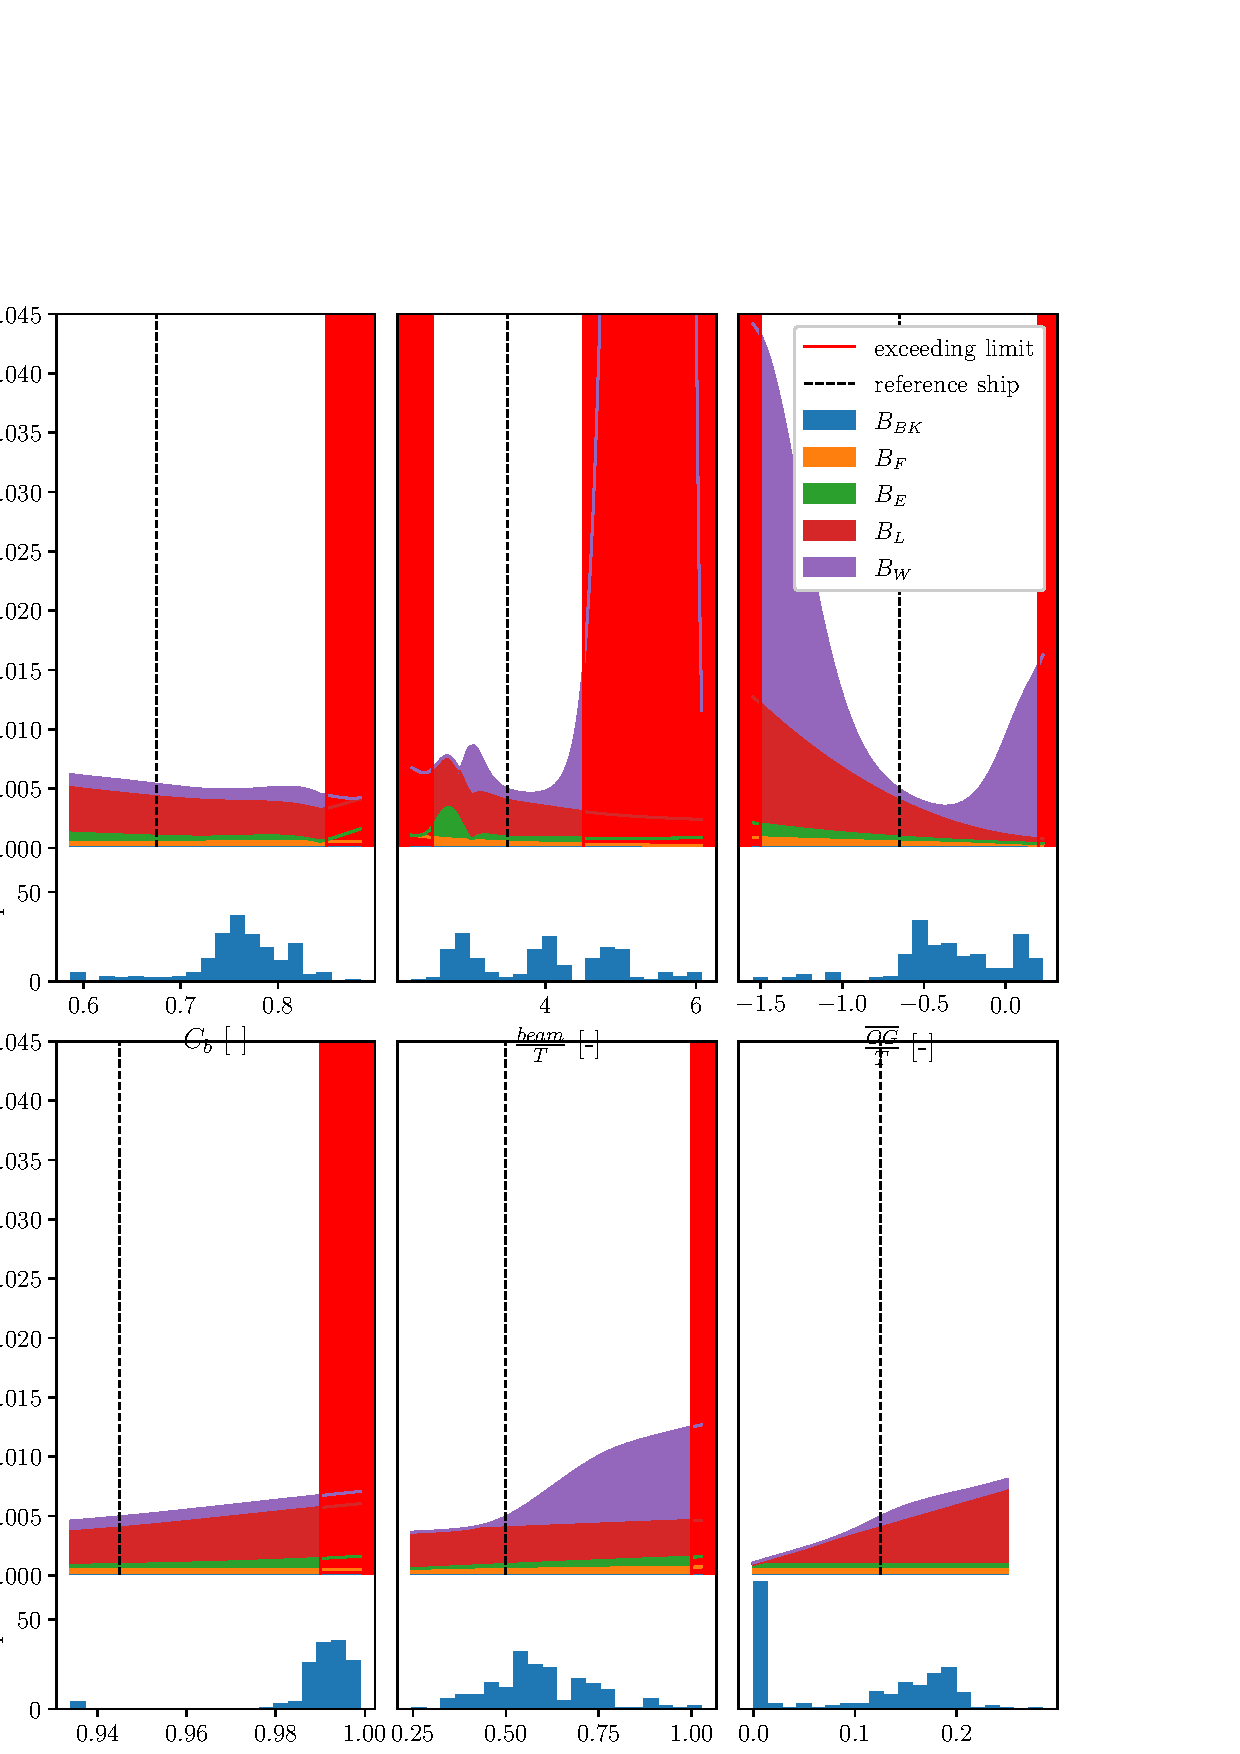
\includegraphics[width=6in, height = 8in ]{figures/SI-sensitivity.pdf}
        \vspace{-0.5cm}
    \caption{SI-method input parameter variation and data base ships}
    \label{fig:SI_sensitivity}
\end{figure}

\subsection{Overall accuracy of Ikeda\'s method}
\label{se:overall_comparison}
In the following, we will present an overall comparison between Ikeda\'s method and the damping estimated from experimental test database in order to identify possible potential to improve Ikeda\'s method.


Figure \ref{fig:B_e_hat_ikeda} shows a comparison of the nondimensional equivalent linear damping from model tests and the simplified method.  

\begin{figure}[H]
    \centering
    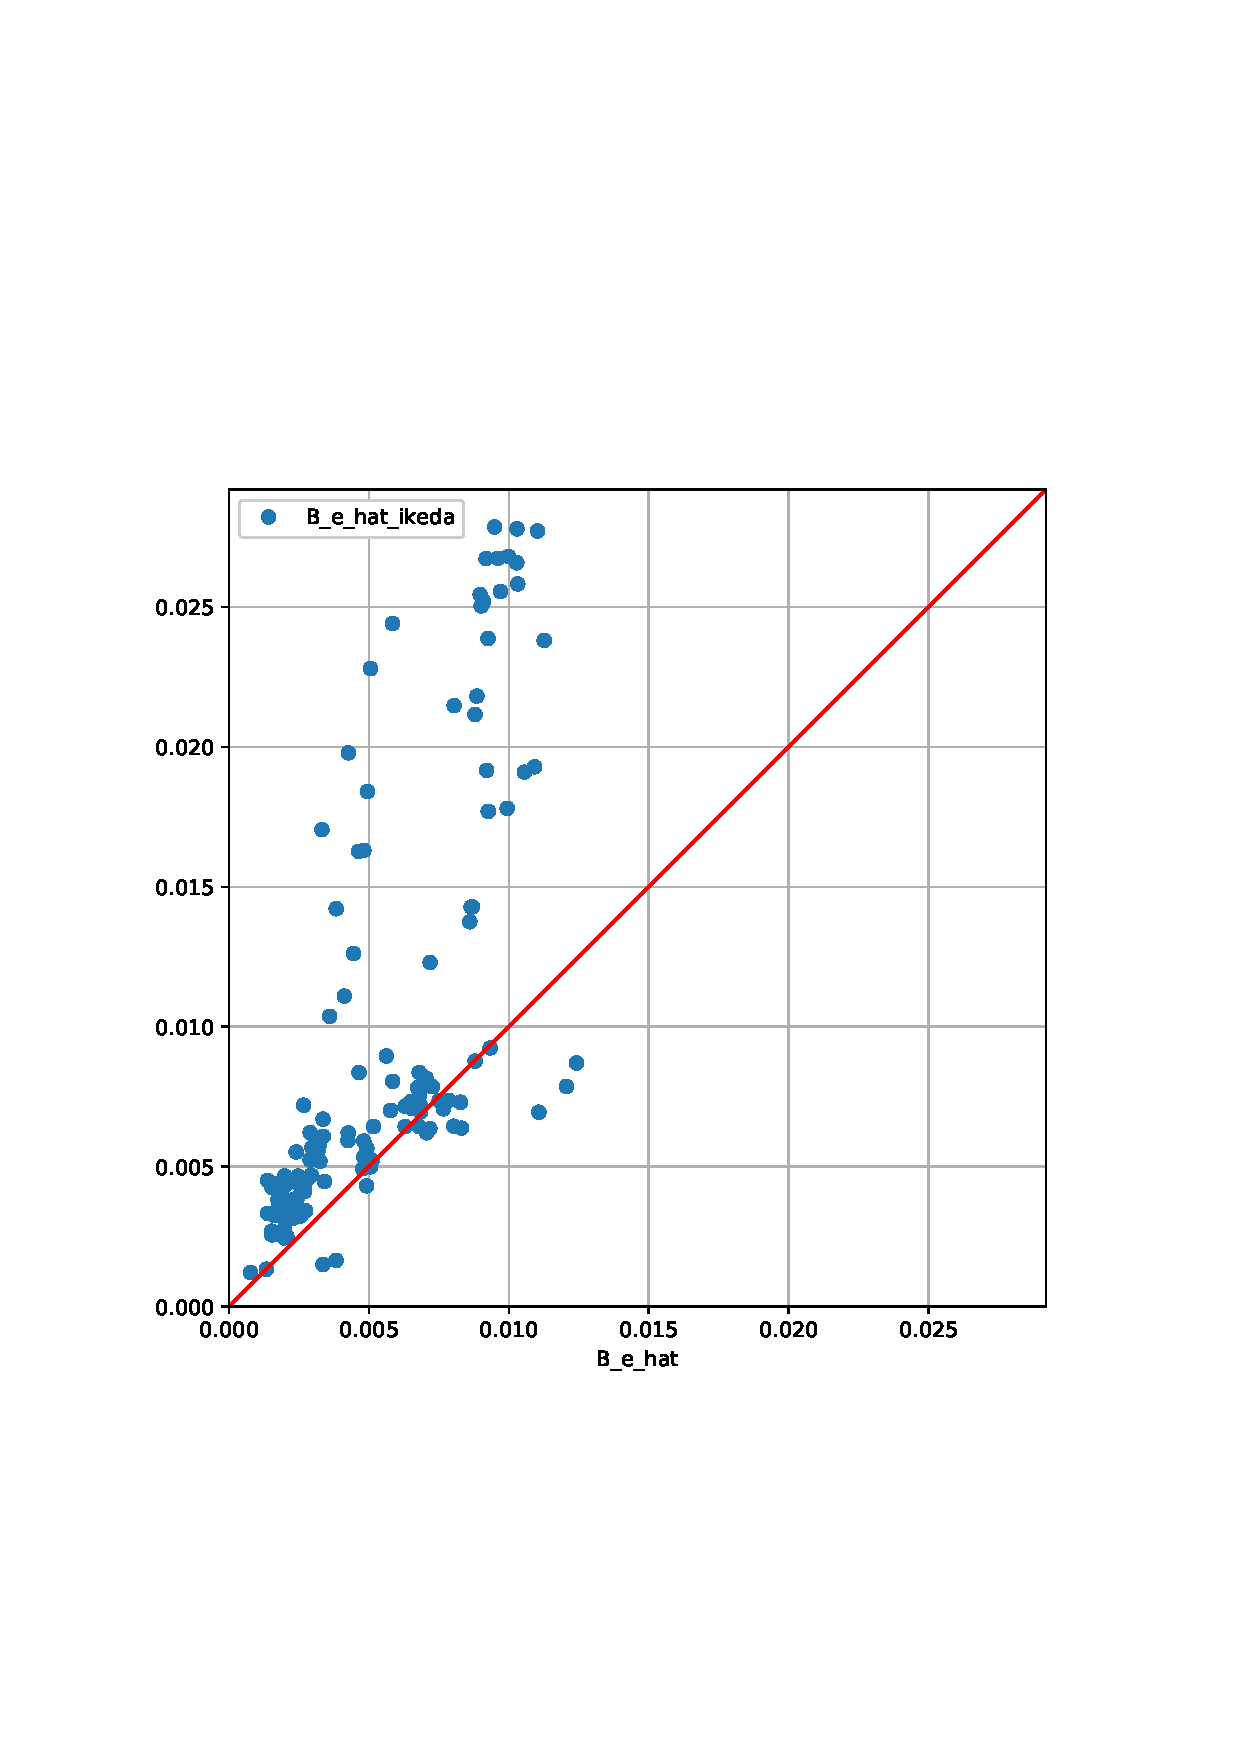
\includegraphics[width=\columnwidth]{figures/B_e_hat_ikeda.pdf}
    \caption{Nondimensional linearized damping from model tests and simplified Ikeda}
    \label{fig:B_e_hat_ikeda}
\end{figure}

When plotting the error between the model test and simplified Ikeda method in figure \ref{fig:B_e_hat_error} this shows that the error is much larger for $T/L_{pp}<0.034$

\begin{figure}[H]
    \centering
    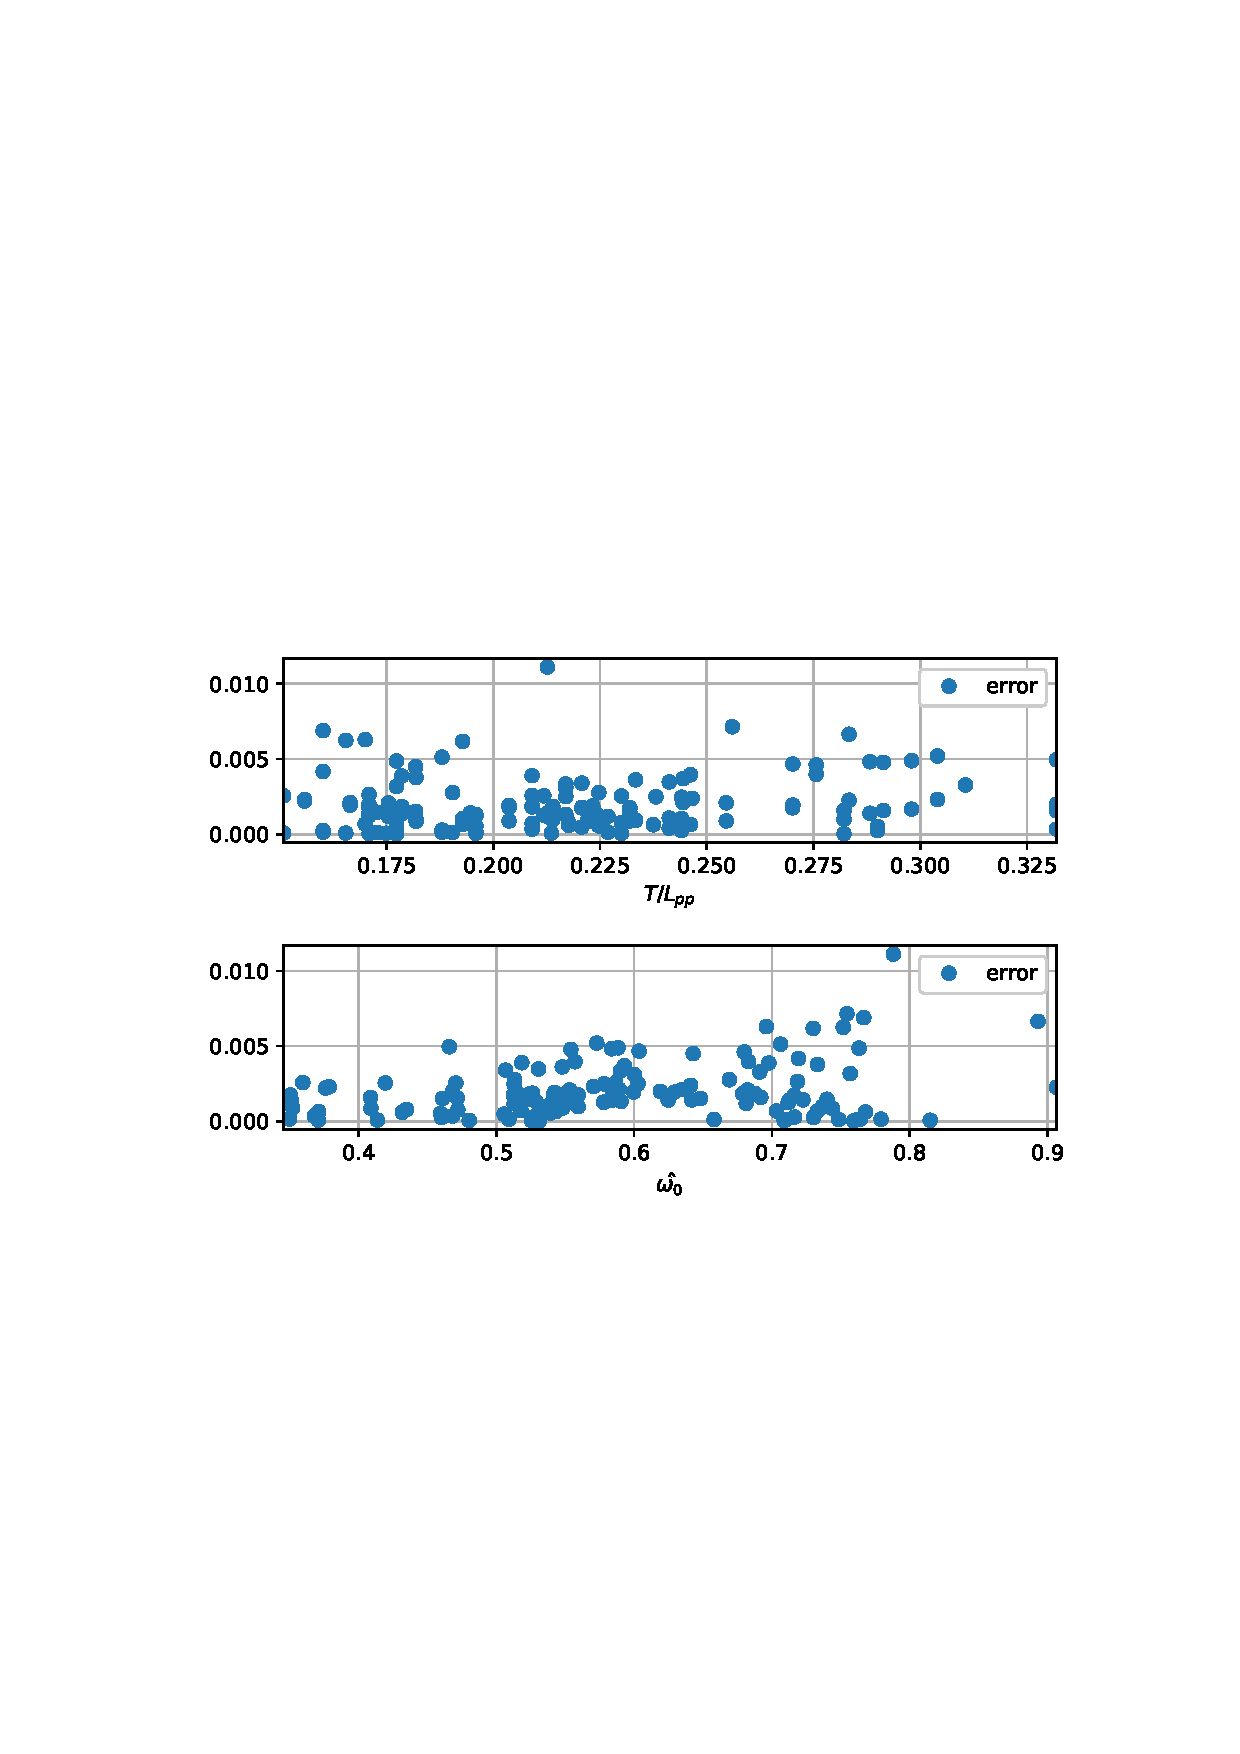
\includegraphics[width=\columnwidth]{figures/B_e_hat_error.pdf}
    \caption{Simplified Ikeda error versus draught}
    \label{fig:B_e_hat_error}
\end{figure}

Figure \ref{fig:B_e_hat_good} shows the comparison for only model tests with $T/L_{pp}>0.034$.
This confirms the small draft to beam ratio limit of this method as mentioned in \cite{kawahara_simple_2011}. The corresponding $R^2$ score is 0.38.

\begin{figure}[H]
    \centering
    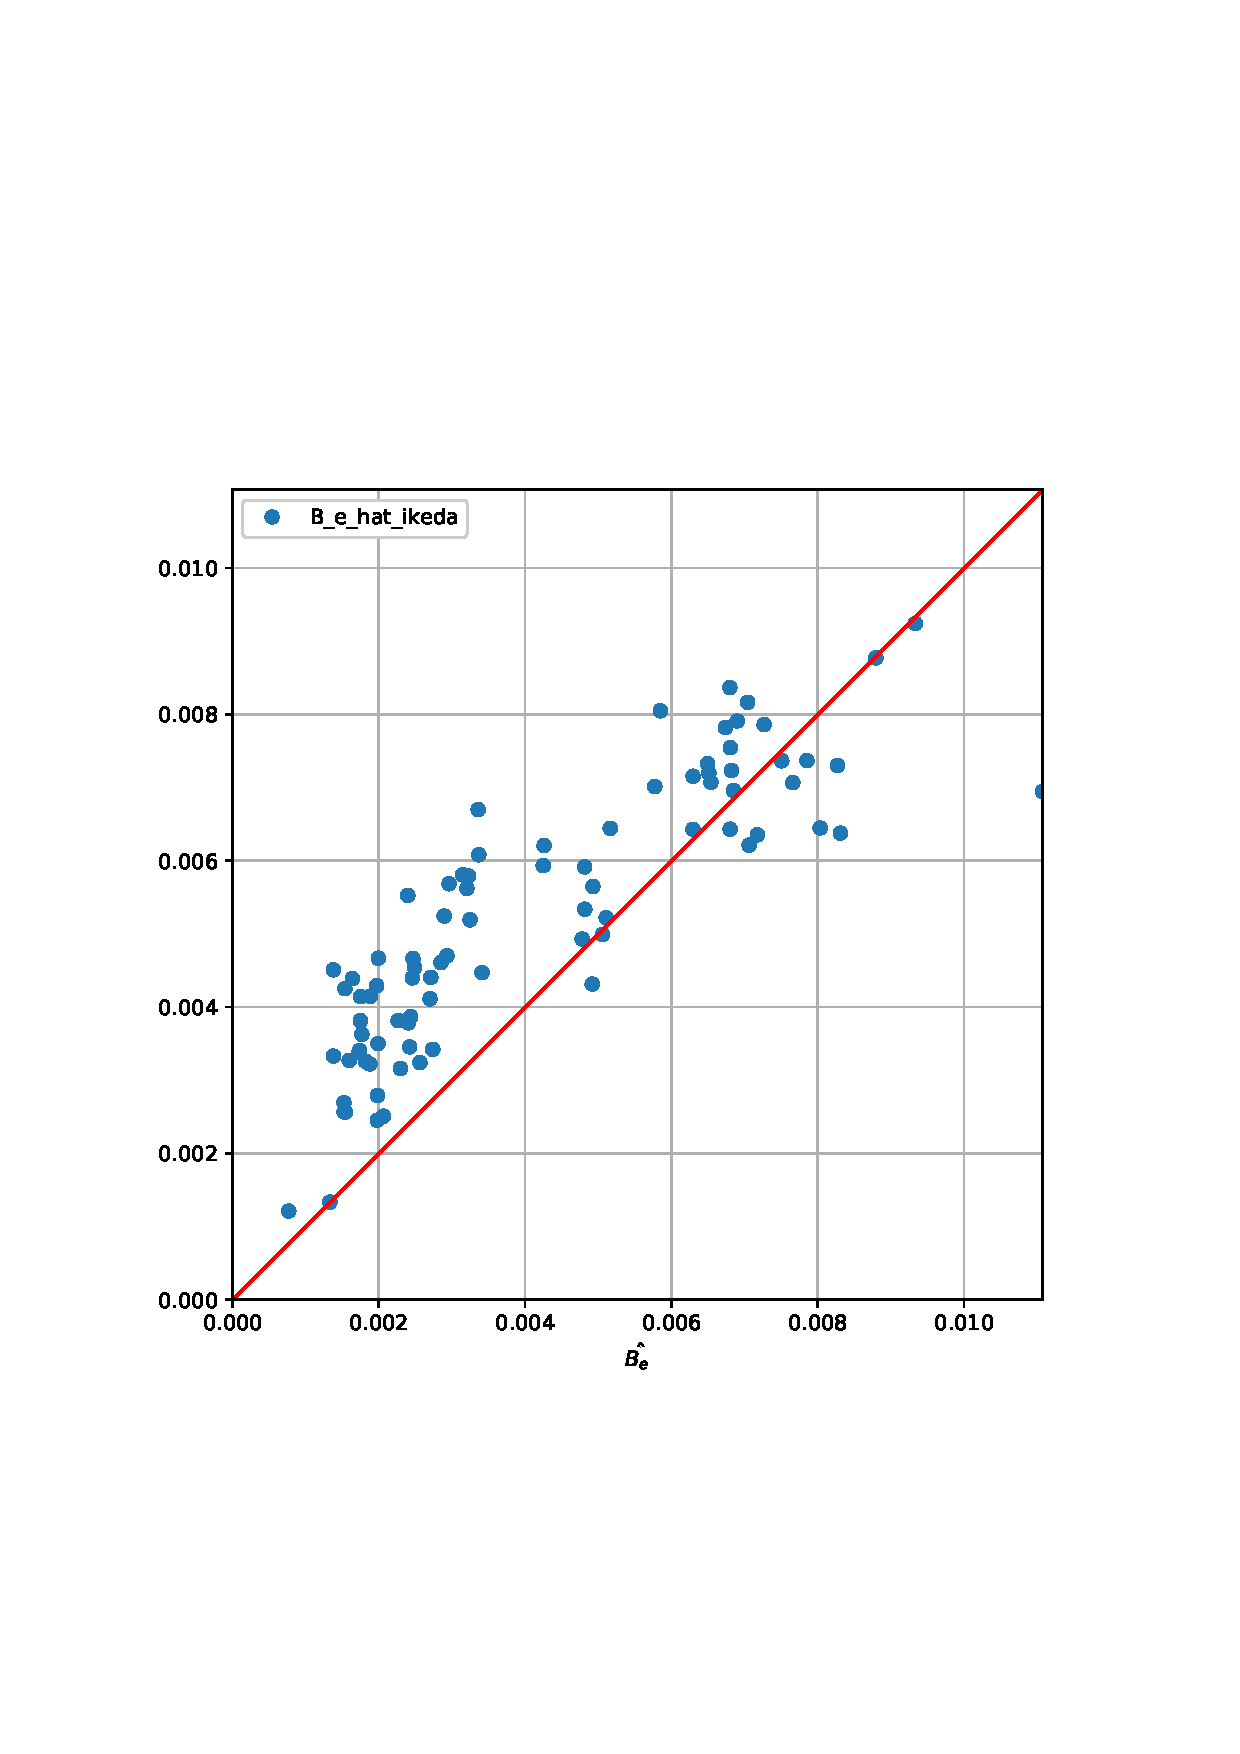
\includegraphics[width=\columnwidth]{figures/B_e_hat_good.pdf}
    \caption{Nondimensional linearized damping from model tests and simplified Ikeda $T/L_{pp}>0.034$}
    \label{fig:B_e_hat_good}
\end{figure}

\section{ML-method for prediction of roll damping}
\label{se:regression} 

Work has been conducted to propose a correction to the SI-method based on the findings in this paper. The idea is to find correction factors that can be applied to the roll damping components calculated with the SI-method. In order to handle the problem of $\hat{B_e}$ accuracy being very much depending on the roll amplitude a roll amplitude correction factor has also added. The correction factors have been determined by fitting a linear regression model to the roll damping components, calculated with the SI-method at roll amplitudes between 0 and 10 degrees, giving the following expression: 
\begin{equation} \label{eq:polynom_correction}
\hat{B_{e}} = 0.7396 \hat{B_{BK}} - 1.256 \hat{B_{E}} + 9.289 \hat{B_{F}} + 0.6891 \hat{B_{L}} + 0.6691 \hat{B_{W}} + 0.02178 phi_{a} - 0.003594
\end{equation}

The proposed correction factors reduce $\hat{B_{BK}}$ and $\hat{B_{W}}$, removes $\hat{B_{E}}$ and $\hat{B_{L}}$ is not corrected much. 

\subsection{Cross validation}
When constructing a regression model from a data set, over-fitting the data can be a problem. Including too many parameters and/or allowing too high order of the model would give a very good representation of the present roll damping data, but large extrapolation errors when the model is used on other data. K-fold cross validation has been used to "mimic" this situation. The data has been split into five smaller sets (folds). Four of the folds are used to train the model and the fifth is used for testing (validation). The validation is done by calculating the coefficient of determination $R^2$ for the fitted model. This is done for all five possible train/test combinations. Applying the proposed correction improves the accuracy according to the cross validation results in table \ref{tab:crossvalidation} with an average $R^2$ of 0.68 compared to 0.47 without the correction. The improvement can also be seen when comparing figure \ref{fig:ikeda_components} with \ref{fig:ikeda_phi_a}.
\begin{tabular}{lrr}
\toprule
{} &  \$R\textasciicircum 2(SI-method)\$ &  \$R\textasciicircum 2(SI-corrected)\$ \\
\midrule
0 &              0.39 &                 0.66 \\
1 &              0.56 &                 0.71 \\
2 &              0.47 &                 0.66 \\
3 &              0.32 &                 0.69 \\
4 &              0.59 &                 0.66 \\
\bottomrule
\end{tabular}


\begin{figure}[H]
\vspace{-0.5cm}
\centering
  \centering
  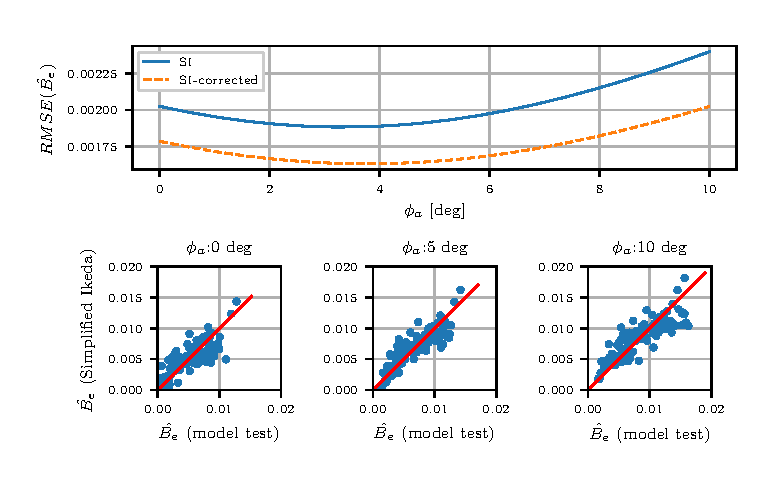
\includegraphics[]{figures/ikeda_corrected_phi_a.eps}
  \vspace{-0.5cm}
  \caption{Root mean square error of roll damping prediction between the SI-method, corrected SI-method and the model test results (upper plot). Influence of roll amplitude $\phi_a$ on $\hat{B_e}$ between the corrected SI-method and model tests for $0^{\circ}$ (bottom left plot), $5^{\circ}$ (bottom middle plot) and $10^{\circ}$ (bottom right plot), respectively.}
  \label{fig:ikeda_phi_a_correction}
\end{figure}

\section{Conclusions}
\label{se:conclusions}

The roll damping database has been compared with predictions with the implementation of the Simplified Ikeda method. The database and the predictions show agreement for some cases (see figure \ref{fig:B_e_hat_good}) but poor agreement for other cases, especially for small draft to beam ratios, typically for Ballast loading condition for many modern ships. It seems that exceeding the limits of the the Simplified Ikeda method will give poor results. These limits are unfortunately not so well defined in \cite{kawahara_simple_2011}. The comparison in the present paper suggest a lower limit of the draught to length ratio of $T/L_{pp}>0.034$.



A regression model has been developed with a little bit better agreement, but still with quite much errors. It seems that more advanced methods, original Ikeda method with strip calculations, CFD or model testing, to predict roll damping is still a better option to get reliable predictions.  



\section*{Acknowledgements}
\label{se:acknowledgements}

\begin{itemize}
    \item Trafikverket (Swedish Transport Administration)
    \item Lighthouse
    \item Sune Thorsson who has collected the meta data about the tested ship models.
\end{itemize}





\section{References}
\label{sec:references}

\bibliographystyle{unsrt}
%\bibliographystyle{abbrvnat}
\bibliography{references}


\end{document}
